\documentclass[tikz,border=2pt]{standalone}
\usepackage{amsmath,amssymb}
\usepackage{pgfplots}
\pgfplotsset{compat=1.18}
\usetikzlibrary{calc}

\begin{document}
% The smoothness ladder: |x| is continuous but not C^1 (kink), x|x| is C^1 but not C^2 (its
% derivative 2|x| has a kink), x^2 is C^2 (and smoother).
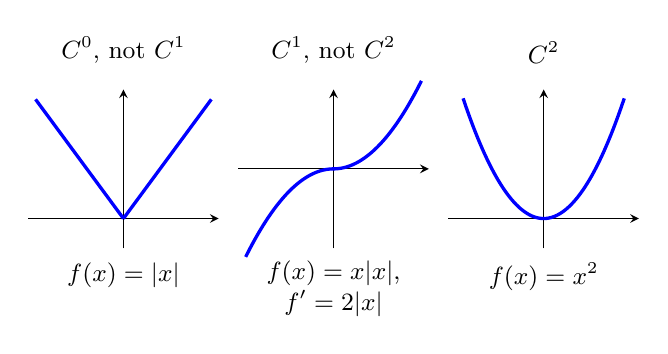
\begin{tikzpicture}
	\begin{axis}[name=p1, axis lines=middle, xmin=-1.3, xmax=1.3, ymin=-0.3, ymax=1.3, xtick=\empty, ytick=\empty, samples=60, width=4.0cm, height=3.6cm, clip=false, title={$C^0$, not $C^1$}, title style={font=\small}]
		\addplot[blue, very thick, domain=-1.2:0, samples=2] {-x};
		\addplot[blue, very thick, domain=0:1.2, samples=2] {x};
		\node[font=\small, anchor=north] at (axis cs:0,-0.35) {$f(x)=|x|$};
	\end{axis}
	\begin{axis}[name=p2, at={(p1.east)}, anchor=west, xshift=0.25cm, axis lines=middle, xmin=-1.3, xmax=1.3, ymin=-1.3, ymax=1.3, xtick=\empty, ytick=\empty, samples=80, width=4.0cm, height=3.6cm, clip=false, title={$C^1$, not $C^2$}, title style={font=\small}]
		\addplot[blue, very thick, domain=-1.2:1.2] {x*abs(x)};
		\node[font=\small, anchor=north, align=center] at (axis cs:0,-1.35) {$f(x)=x|x|$,\\ $f'=2|x|$};
	\end{axis}
	\begin{axis}[name=p3, at={(p2.east)}, anchor=west, xshift=0.25cm, axis lines=middle, xmin=-1.3, xmax=1.3, ymin=-0.3, ymax=1.3, xtick=\empty, ytick=\empty, samples=80, width=4.0cm, height=3.6cm, clip=false, title={$C^2$}, title style={font=\small}]
		\addplot[blue, very thick, domain=-1.1:1.1] {x^2};
		\node[font=\small, anchor=north] at (axis cs:0,-0.35) {$f(x)=x^2$};
	\end{axis}
\end{tikzpicture}
\end{document}
